\part{Seminar 1 - A Generalized Magnetic Circuit Modeling Approach for Design of Surface Permanent-Magnet Machines}

\makebox[.25\textwidth]{Dylan De Coeyer}\makebox[.25\textwidth]{Gauthier De Coninck}\makebox[.25\textwidth]{Amandine Demarcin}\makebox[.25\textwidth]{Guillaume Derycke}

\section*{Abstract}
The paper proposes a generalized equivalent magnetic circuit model for the design of permanent-magnet (PM) electric machines, taking saturation into account without the need for finite-element analysis (FEA).

\section{Introduction}
\paragraph{Slides 1 to 5} Rare earth permanent magnet (PM) brushless machines possess the features :
\begin{itemize}
    \item high efficiency
    \item high torque / power density
    \item low maintenance
\end{itemize}
which makes them excellent candidate for :
\begin{itemize}
    \item electric vehicles
    \item wind turbines
    \item marine energy converters
\end{itemize}
The \textbf{equivalent magnetic circuit model (EMCM)} is a common technique for the design of electric machines, with the following drawbacks :
\begin{itemize}
    \item excessive simplification
    \item lack of accuracy to predict flux saturation
    \item lack of accuracy to predict machine performance with any pole-slot count
\end{itemize}
For those reasons, EMCM is used for \textbf{preliminary design}.

\textbf{Finite-element analysis (FEA)} can directly calculate the flux patterns, but :
\begin{itemize}
    \item The entire process is computationally expensive
    \item A change in the parameters often implies a model reconstruction
    \item Some configurations make it difficult to reduce the computational time
\end{itemize}
For those reasons, FEA is unsuitable for preliminary design, but might be used for \textbf{design verification}. 

\paragraph{Conclusion} A universal EMCM is necessary for rapid accurate machine design of general PM machines. The existing literature rarely considered the detailed model for PM poles contribution to the flux in each tooth for any relative position of the rotor and stator.

\paragraph{Proposed model}
\begin{itemize}
    \item Takes pole-slot count and flux saturation into account
    \item Employs a circular configuration
    \item Ensures that the flux pattern of machines with any pole-slot counts and winding can be calculated
    \item Magnets (MMF sources) are virtually modularized into several segments to associate with stator slots (major contribution of this paper)
    \item Applicable to any pole-slot combinations, more generalized
\end{itemize}

\section{The magnetic model}
\subsection{Definitions}
\paragraph{Slides 6 to 14}

This section discusses the modeling of PMs in a PM machine by considering stator slots/teeth and rotor position. Flux leakage occurs when the flux produced by a magnet fails to flow through the stator windings and thus contributes no magnitude to the back electromotive force (EMF). The level of flux leakage depends on :
\begin{itemize}
    \item pole-to-slot ratio
    \item slot geometric features
    \item rotor position
\end{itemize}

Three conditions are considered here, depending on the rotor position :
\begin{itemize}
    \item \textbf{Flux cancellation} mode accounts for the most serious flux leakage, as shown in Fig. \ref{2.3}(a)
    \item \textbf{Partial contribution} mode, part of one pole is within a slot pitch : the contribution of flux from the magnet is mitigated (Fig. \ref{2.3}(b))
    \item \textbf{Full contribution} mode in Fig. \ref{2.3}(c), the whole slot pitch is covered by one pole, where all the flux produced by the magnet is treated as flowing through the tooth.
\end{itemize}

\begin{figure}[H]
    \centering
    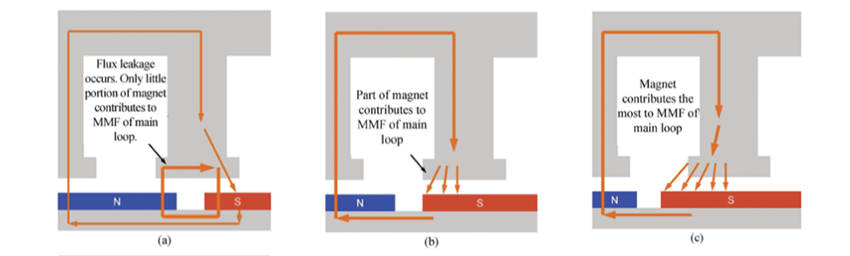
\includegraphics[width = 0.8\textwidth]{2_3.png}
      \caption{Flux distributions : (a) Flux cancellation, (b) partial contribution, and (c) full contribution.}
      \label{2.3}
\end{figure}

The \textbf{slot pitch} $\theta_S$ is shown in Fig. \ref{2.4}. It is assumed that the contribution of the magnet to MMF is proportional to the portion of the magnet within $\theta_S$.

\begin{figure}[H]
    \centering
    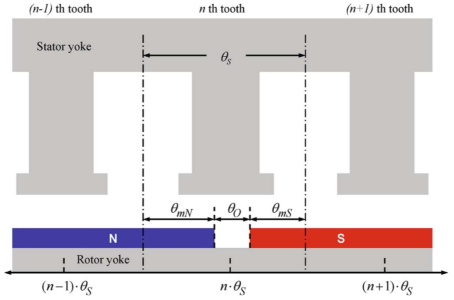
\includegraphics[width = 0.5\textwidth]{2_4.png}
    \caption{Features of magnet within a slot pitch}
    \label{2.4}
\end{figure}

The effective portion of the magnet in a slot pitch, considering flux leakage, can be expressed as $$\theta_{eq} = C_m \cdot \theta_S $$ where $C_m$ is defined as the \textbf{effective magnet factor} for a tooth / segment and can be defined as
tooth/segment and can be defined as $$C_m = \frac{\theta_{mN}-\theta_{mS}}{\theta_S}, \ -1 \leq C_m \leq 1$$
It is necessary to calculate $C_m$ for every single tooth or segment to determine the coil flux linkage. $C_m$ can therefore be written as a function of the nth tooth : $C_m = C_m(n)$. Here are the steps to find $C_m$ :
\paragraph{1) Calculation of Slot Pitch} The slot pitch in electrical degrees can be written as $$\theta_S = \frac{360}{N_S} \cdot \frac{N_m}{2}$$ where $N_m$ is the number of poles and $N_s$ is the number of slots.
\paragraph{2) Calculation of Relative tooth angle}
The relative slot angle $\theta_{sl}(n)$ to a reference for the $n$-th \\tooth/segment in electrical degrees is defined as $$\theta_{sl}(n)=(n-1) \cdot \theta_S + \alpha \cdot \frac{N_m}{2}, \ n=1,2,3,\dots,N_s$$
where $\alpha$ is the mechanical angle between a reference on the stator and the first tooth. \textbf{Pay attention, in the paper, there is no mention of the angle $\alpha$. It seems weird for us because, without this angle, the rotor doesn't turn. So added it.}\\
For simplification, we use the remainder which can be expressed as $$\theta_r(n) = Rem\{\theta_{sl}(n),360\degree\}$$
\paragraph{3) Magnet Polarity Associated With Tooth/Segment}
The sign of $\theta_r(n)$ in (6) is used to recognize the polarity of the magnet (+ for N-pole and - for S-pole)
$$
Sign(\theta_r(n)) = \left\{
    \begin{array}{ll}
        1 & \theta_r(n) \leq 180\degree \\
        -1 & \mbox{otherwise.}
    \end{array}
\right.
$$
\paragraph{4) Rearrangement of Relative Tooth Angle}
Because $\theta_{sl}(n)$ has a period of $360\degree$ E, it can be treated within the range of $\pm 180\degree E$ $$\theta_r(n) = Rem\{\theta_{sl}(n)+180\degree,360\degree\}-180\degree$$
\paragraph{5) Determination of $C_m(n)$}
$$
C_m(n) = \left\{
    \begin{array}{ll}
        Sign(\theta_r(n)), & Re\{e^{j\theta '_{s1}(n)}\}\leq b \\
        Sign(\theta_r(n)) \cdot \Big[1-\frac{\frac{\theta_S-\theta_O}{2}-|\theta '_{s1}(n)|}{\theta_S} \Big], & b \leq Re\{e^{j\theta '_{s1}(n)}\}\leq a \\
        Sign(\theta_r(n)) \cdot \frac{2|\theta '_{s1}(n)|}{\theta_S}, & Re\{e^{j\theta '_{s1}(n)}\}\geq a
    \end{array}
\right.
$$
with $$a=Re\Big\{e^{j(\frac{\theta_S-\theta_O}{2})}\Big\} \text{ and } b=Re\Big\{e^{j(\frac{\theta_S+\theta_O}{2})}\Big\} $$

\begin{figure}[H]
    \centering
    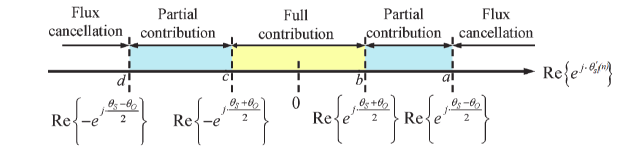
\includegraphics[width=0.8\textwidth]{Flux_contrib.png}
    \caption{Boundaries of the modes on the real axis.}
    \label{fig:boundaries}
\end{figure}
\begin{figure}[H]
    \centering
    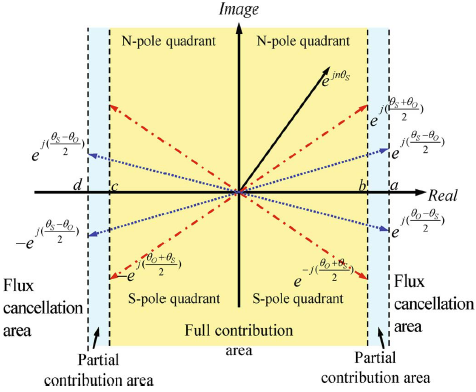
\includegraphics{Flux_contrib2.png}
    \caption{Modified slot angle $\theta_{sl(n)}$ on polar-coordinate plane.}
    \label{fig:modified_slot_angle}
\end{figure}

\subsection{Reminders}

\paragraph{Slide 16}
Analogy between Ohm's law for electrical circuits and Hopkinson's law for magnetic circuits (cfr Figure \ref{fig:Hopkinson}).
\begin{figure}[H]
    \centering
    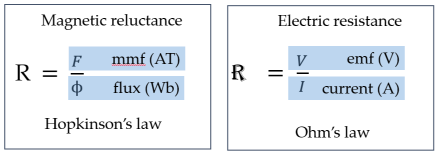
\includegraphics[scale=0.5]{Ohm_Hopkinson.png}
    \caption{Analogy Ohm - Hopkinson}
    \label{fig:Hopkinson}
\end{figure}

\paragraph{Slides 17 to 20}
Derivation of the magnetic circuit model for each element of the machine.

\paragraph{Slide 17: Iron}
%Assumptions:
%\begin{itemize}
%    \item Iron pieces have constant section
%    \item The flux is homogeneous on the section
%    \item No leakage
%\end{itemize}
In a ferromagnetic material, there is a linear relationship between B and H.
The 3 assumptions enable us to link B and the flux $\phi$.
We inject these two relations into the definition of the MMF across the iron section.
Then, by identification with Hopkinson's law, we find the expression of the magnetic reluctance of iron.

\paragraph{Slide 18 and 19: Permanent magnet}
Here the relation between B and H is different since the magnet produces some MMF on its own.
Then the reasoning is the same as for iron.

Another analogy between electrical and magnetic circuits: Thévenin and Norton equivalent circuits. So the permanent magnet can also be represented by a reluctance in parallel with a source of flux. We will use this representation in the seminar.

\paragraph{Slide 20: Solenoid}
From Ampere's law, we find that the MMF induced by the solenoid is independant of the flux, so we model it as a constant source.

\subsection{Application}

\paragraph{Slide 21 and 22}
Knowing the general shape we cut the whole machine (seen as a magnetic circuit) into several parts with a simple geometry… (\autoref{fig:reluctance_couleur}). We will for instance transform the bottom of each slot (that we call the stator yoke) into a reluctance, the teeth’s into a order, etc 
Notice that some reluctance are fixed and others are variables since the expression of the reluctance depend on the permeability that depends on the working point ! $R=\cfrac{l}{\mu \cdot A}$.
We combine those simple elements in a circuit that is representative of our machine. $F_{s,i}$ is the MMF source representing the coil on tooth i.
This is why the technique is named \textbf{EMCM}: Equivalent Magnetic Circuit Model.

\begin{figure}[h!]
    \centering
    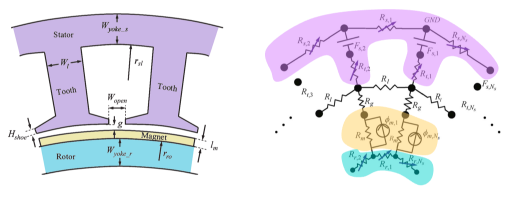
\includegraphics[width=\textwidth]{reluctance_couleur.png}
    \caption{Portion of the machine transformed into a reluctance net.}
    \label{fig:reluctance_couleur}
\end{figure}

\paragraph{Slides 23 to 28}
Now that the topology is fine, we choose the values of the elements of the circuit according to the physics of the machine (dimensions, ...)
The only important formula is :
$$ R = \cfrac{l}{\mu A}$$

Notice that on \textbf{slide 28} the fringing effect between the different teethes is taken into account (the formula is not demonstrated).


\subsection{Formalism}

How to solve this circuit? Write equations.
We want the model to be very generic, so notations are heavy.
We want to find something of the form:
$$x=A^{-1}z$$
With x the unknowns and z the source terms.
\paragraph{Slide 30: Unknowns}
$N_s$ is the number of teeth. We have 5 nodes per branch, but only $5 N_s-1$ unknown nodes because one of them is the reference (GND).

\paragraph{Slide 31: Source terms}
Flux from the magnets: $\phi_m = B_r A$, as shown in slide 19.
$\tau_{mag}$ takes non-idealities of the magnets into account. (e.g. laminated magnets)
$C_m$ is the coupling factor taking the relative position of teeth and magnets into account.

Bottom part of the vector: MMF source terms coming from the coils.

\paragraph{Slides 32 and 33}
We link unknowns and source terms with equations by applying Hopkinson's law in the circuit.
The equations are grouped as heavy submatrices.
\textbf{G} itself is made of submatrices.

\textbf{Erratum!} In slide 32, the matrices' dimensions are wrong. The correct dimensions are in Figure \ref{fig:matrix}.

\begin{figure}[H]
    \centering
    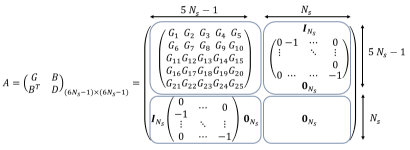
\includegraphics[scale=0.6]{Matrix_dim.png}
    \caption{Matrix A and constituting submatrices}
    \label{fig:matrix}
\end{figure}

\subsection{Operating point}

We have solved the equation $x=A^{-1} z$, so we know the MMF at all nodes and the flux in the coils.
From this information we can find the fluxes everywhere in the machine by applying Hopkinson's law.
\textbf{Some equations were wrong in the paper, what is written in the slides is correct.}

\paragraph{Slide 35}
Be careful with the numbering of different nodes. Branch n=1 corresponds to index 0 of node names.

\paragraph{Slides 37 and 38}
Need to define ''par partie'' because we refer to the reference node (GND) differently from other nodes We have directly set this value to 0.

\paragraph{Slide 39}

Development of the expressions of the slide :

\begin{minipage}[t]{0.45\linewidth}
\begin{align*}
    B_{m,n} & = \frac{\phi}{A}\\
    & = \frac{\Delta F}{A R}
\end{align*}
\end{minipage}
\begin{minipage}[t]{0.45\linewidth}
\begin{align*}
    H_{m,n} & = \frac{B}{\mu}\\
    & = \frac{\Delta F}{A R} \frac{1}{\mu} \\
    & = \frac{\Delta F}{A} \frac{\mu A}{l} \frac{1}{\mu}\\
    & = \frac{\Delta F}{l}
\end{align*}
\end{minipage}

\begin{figure}[H]
    \centering
    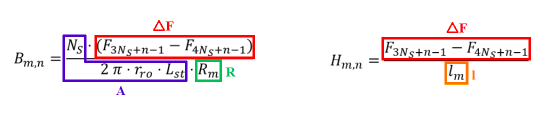
\includegraphics[width=0.8\textwidth]{equ.png}
\end{figure}

\section{The equivalent magnetic circuit model}

\section{Iterative calculation}

\paragraph{Slides 41 to 43: Iterate to take the non-linearity of the material into consideration}
The principle is to start from an arbitrary value of relative permeability (4000) that allows to calculate a first EMCM that gives a flux and thus a flux density:
$$B_{new} = \cfrac{\phi_{new}}{A}$$
And knowing the B-H profile and the definition of the permeability to calculate a second EMCM... :
$$\mu_{new}=\cfrac{\Delta B_{new}}{\Delta H_{new}}$$

\paragraph{Slides 44 to 49: Understand the iteration schematic}
We analyse the machine for ONE SINGLE ROTOR POSITION.
We can assume that if all conditions are met for this position, they should be ok for other positions too.
But we will need to check, and if it doesn't match the whole design must be restarted.

All input parameters (slide 44) allow us to find the values for all components in the magnetic circuit.
Reluctances are used to compute matrix A, source terms are used to compute vector z in equation $x= A^{-1} z$.
Then we can solve this equation and find x (slide 45).
Knowing x, we use these values to find the flux in all parts of the machine (slide 47).
Since we also know the magnetic characteristic of the materials, from the flux we find the magnetic intensity in the machine (slide 48).
We want the material to be saturated, so we check if it is the case. If not we change the dimensional parameters to reduce the amount of iron used (slide 49).

\paragraph{Slide 50: Why is saturation wanted?}
Saturation means that I need to increase excitation current intensity a lot to improve the magnetic flux a little.
If I reduce the section of the teeth, saturation will be reached sooner, but I have more space in the slots to put wire, and increase the number of turns.
So there is a trade-off between saturation and number of turns I can put in my machine.
Obviously, the authors found that the optimum lies a little above the saturation limit.

\section{Use of the EMCM}

\paragraph{Slide 52-53: Reminder}
The torque in a electrical machine can have 3 different origins as we see on \autoref{fig:couple_couleur}:
\begin{itemize}
    \item the first term represent the \textbf{detent torque} that try to align the stator and rotor saliencies, caused by the flux of permanent magnets. 
    \item The second term is the \textbf{electrodynamic torque} that roughly speaking  comes from Lorenz’s law.
    \item The third one is the \textbf{reluctant torque} that is a bit similar to the detent torque but with coils.
\end{itemize}
\begin{figure}[h!]
    \centering
    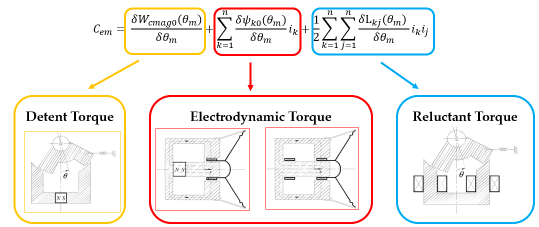
\includegraphics[width=0.6\textwidth]{couple_couleur.png}
    \caption{Caption}
    \label{fig:couple_couleur}
\end{figure}

In our case we only care about \textbf{round-rotor} machines (without any salience's). So have only an electrodynamic torque !

\paragraph{Slide 54-55: Getting the power}
The torque multiplied by the angular velocity gives a power:
$$P_{meca} = C_{em} \cdot \omega = \sum_{k=1}^3 \cfrac{\delta \psi_{k0}(\theta_m)}{\delta \theta_m} i_k \cdot \omega $$
Where the term: $\cfrac{\delta \psi_{k0}(\theta_m)}{\delta \theta_m} \ \cdot \omega $ is the Back-EMF term.

\paragraph{Slide 56-57: other features}
If we are able to calculate the flux when the current in some winding's is null (by imposing a zero MMF in some source from the magnetic model) we can calculate inductance coefficients. \\
Knowing all theses information's we can retrieve the tensions by :
$$ u_k =  R_k i_k + L \cfrac{d i_k}{d t} + \cfrac{\delta \psi_{k0}}{\delta \theta} (\theta)$$


\section{Results}

\paragraph{Slides 59 to 60} Experimentation is necessary to verify the good behavior of the model. A set of parameters has been used as input in order to design a 540kW machine. Using the iterative process described in Section 4, a set of output parameters have been obtained. These parameters are mostly geometrical, like the pole number, slot number, number of turns per coil, parallel paths, and other dimensions. We see also information about the air-gap flux density, as well as information about magnets. $B_r$ is the residual magnetization of the magnet when the external field intensity is null. $H_{cb}$ is the external field required to counteract the magnetic field of the magnet, while $H_{cj}$ is the field required to demagnetize the magnet.

\paragraph{Slide 61} A comparison will be made between straight and skewed rotor. A skewed rotor is just a rotor whose magnets are inclined. The skew can be continuous, or discontinuous as can  be seen on the experimental setup.

\paragraph{Slide 62} The back-EMF is computed using the magnetic model, and compared to finite-element methods for a skewed and a straight rotor. At first sight, we observe that the evolution of back-EMF is much smoother with a skewed rotor, both for EMCM and FEA. It can be explained by the fact that transitions of the magnetic coupling coefficient is much smoother in this case. Then, we can observe that the EMCM gives a very good approximation, even if it tends to oscillate at some position with the straight rotor.

\paragraph{Slide 63} Now, the model results are compared with experimental data. In the same way, we see that the approximation is accurate, but oscillates a bit more than FEA.

As a conclusion, we can say that the developed model is sufficiently accurate for the design of PM machines without the aid of time-consuming FEA.

\section{Conclusion}
\paragraph{Slide 64} What should you remember from this seminar?

First, the purpose was to develop an equivalent magnetic circuit model, faster than FEA, to design and analyse a PM machine. 
What makes this model better than the one conventionally used?
\begin{itemize}
    \item It takes pole/slot and flux saturation into account
    \item It is applicable to any pole-slot combination
\end{itemize}
How is it done?
\begin{itemize}
    \item The PM machine is modeled as a reluctance network
    \item Fluxes and MMFs are computed via matrix equation
    \item An iterative process is used to optimize the design
    \item The electromotive torque, power, back-emf can then be computed
\end{itemize} 
